\documentclass[uplatex, twocolumn,12pt]{jsarticle}

% 縦横のサイズ調整
\usepackage[top=10mm, bottom=10mm, left=10mm, right=10mm]{geometry}
\usepackage[dvipdfmx]{graphicx}
\usepackage{latexsym}
\usepackage{bmpsize}
\usepackage{url}
\usepackage{comment}

\begin{document}


\title{\vspace{-10mm}InputMethodKitとTCAを使ったmacOS上で動作するIMEの開発}
\author{Tatsumi0000}
\date{}
\maketitle


\section{はじめに}
% \begin{figure}[t]
%     \begin{center}
%         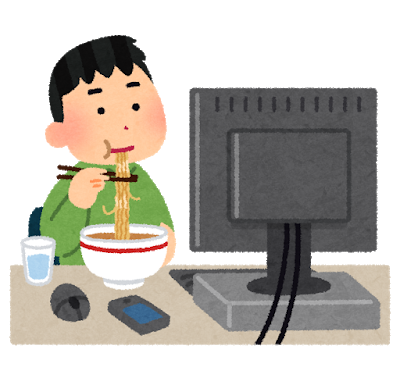
\includegraphics[width=7cm]{image/syokuji_computer.png}
%         \caption{パソコンの前でご飯を食べる人のイラスト}
%         \label{fig:syokuji_computer}
%     \end{center}
% \end{figure}

パソコンの前でご飯を食べることはよくある。パソコンの前でご飯を食べる人のイラストを図\ref{fig:syokuji_computer}に示す。
このイラストは、規約の範囲内であれば、個人、法人、商用、非商用問わず無料で利用できることでおなじみの、{\bf かわいいフリー素材 いらすとや}\cite{irasutoya}より引用した。

\section{おわりに}
やっぱり{\bf いらすとや}のイラストはすばらしい。

\begin{thebibliography}{99}
    \bibitem{irasutoya} いらすとや, last access 2019.6.13 \url{https://www.irasutoya.com/}



\end{thebibliography}

\end{document}
